%%%%%%%%%%%%%%%%%%%%%%%%%%%%%%%%%%%%%%%%%%%%%%%%%%%%%%%%%%%%%%%%%%%%%%%%%%%%%%%%
% Preámbulo                                                                    %
%%%%%%%%%%%%%%%%%%%%%%%%%%%%%%%%%%%%%%%%%%%%%%%%%%%%%%%%%%%%%%%%%%%%%%%%%%%%%%%%

\documentclass[11pt,a4paper,titlepage,twoside,openright,openbib]{report}

%%% RELACIÓN DE VARIABLES A PERSONALIZAR %%%
%\def\lingua{gal}
\def\lingua{esp} % descomenta esta liña se redactarás a memoria en español
%\def\lingua{eng} % descomenta esta liña se redactarás a memoria en inglés
\def\nome{Diego Trabazo Sardón}                             % substitúe aquí o teu nome
\def\nomedirectorA{José Carlos Dafonte Vázquez}             % substitúe aquí o nome de quen dirixe
\def\titulo{Sistema para la extracción automática de información estructurada a partir de documentos con
elementos de maquetación comunes} % substitúe aquí o título do teu TFG
%\def\mencion{NOME DA MENCIÓN}                        % descomenta a mención correspondente
\def\mencion{COMPUTACIÓN}
%\def\mencion{ENXEÑARÍA DO SOFTWARE}
%\def\mencion{ENXEÑARÍA DE COMPUTADORES}
%\def\mencion{SISTEMAS DE INFORMACIÓN}
%\def\mencion{TECNOLOXÍAS DA INFORMACIÓN}

\def\renomearcadros{si} % descomenta esta liña se redactas a memoria en español e prefires que
                         % os "cuadros" e o "índice de cuadros" se renomeen
                         % a "tablas" e "índice de tablas" respectivamente

\usepackage{estilo_tfg}

% Cambia el tipo y tamaño de la fuente monoespaciada en todo el documento
\setmonofont[Scale=MatchLowercase]{IBMPlexMono}

% Lista de paquetes potencialmente interesantes (uso baixo demanda)

% \usepackage{alltt}       % proporciona o entorno alltt, semellante a verbatim pero que respecta comandos
% \usepackage{enumitem}    % permite personalizar os entornos de lista
% \usepackage{eurofont}    % proporciona o comando \euro
% \usepackage{float}       % permite máis opcións para controlar obxectos flotantes (táboas, figuras)
% \usepackage{hhline}      % permie personalizar as liñas horizontais en arrays e táboas
% \usepackage{longtable}   % permite construir táboas que ocupan máis dunha páxina
% \usepackage{lscape}      % permite colocar partes do documento en orientación apaisada
% \usepackage{moreverb}    % permite personalizar o entorno verbatim
% \usepackage{multirow}    % permite crear celdas que ocupan varias filas da mesma táboa
% \usepackage{pdfpages}    % permite insertar ficheiros en PDF no documento
% \usepackage{rotating}    % permite diferentes tipos de rotacións para figuras e táboas
% \usepackage{subcaption}  % permite a inclusión de varias subfiguras nunha figura
% \usepackage{tabu}        % permite táboas flexibles
% \usepackage{tabularx}    % permite táboas con columnas de anchura determinada
\usepackage{minted} % proporciona código coloreado para el código


%%%%%%%%%%%%%%%%%%%%%%%%%%%%%%%%%%%%%%%%%%%%%%%%%%%%%%%%%%%%%%%%%%%%%%%%%%%%%%%%
% Corpo                                                                        %
%%%%%%%%%%%%%%%%%%%%%%%%%%%%%%%%%%%%%%%%%%%%%%%%%%%%%%%%%%%%%%%%%%%%%%%%%%%%%%%%

\begin{document}

 %%%%%%%%%%%%%%%%%%%%%%%%%%%%%%%%%%%%%%%%
 % Preliminares do documento            %
 %%%%%%%%%%%%%%%%%%%%%%%%%%%%%%%%%%%%%%%%

 \begin{titlepage}
  
  \hspace*{128pt}
  \textcolor{udcpink}{{\fontencoding{T1}\fontfamily{phv}\selectfont Facultade de Informática}}\\[-32pt]

  \begin{center}
    
\includegraphics[scale=0.3]{imaxes/udc}\\[35pt]

    {\large TRABALLO FIN DE GRAO \\
            GRAO EN ENXEÑARÍA INFORMÁTICA \\
            MENCIÓN EN \mencion } \\[100pt]
    
    \begin{huge}
      \begin{spacing}{1.3}
        \bfseries \titulo
      \end{spacing}
    \end{huge}
  \end{center}
  
  \vfill
  
  \begin{flushright}
    {\large
    \begin{tabular}{ll}
      {\bf Estudante:} & \nome \\
      {\bf Dirección:} & \nomedirectora1 \\ % COPIA E PEGA ESTA LIÑA SE O PRECISAS
    \end{tabular}}
  \end{flushright}
  \rightline{A Coruña, \datasimple\today.}
\end{titlepage}

 \paxinaenbranco
 \dedicatoria{Dedicatoria} % escribe neste comando o teu texto de dedicatoria
 \paxinaenbranco
 \paxinaenbranco
 \begin{agradecementos}
 \blindtext                % substitúe este comando polo teu texto de agradecementos
 \end{agradecementos}
 \paxinaenbranco
 %%%%%%%%%%%%%%%%%%%%%%%%%%%%%%%%%%%%%%%%%%%%%%%%%%%%%%%%%%%%%%%%%%%%%%%%%%%%%%%%

\begin{abstract}\thispagestyle{empty}

Este TFG tiene por objetivo la creación de una solución de entorno servidor, para automatizar la adquisición de información desde fuentes de datos semiestructuradas, como son los PDF. El proyecto se enmarca en el ámbito de la transición de organizaciones, públicas o privadas, hacia la informatización de los procesos.
Se centra específicamente en documentos donde existe un modelo común de maquetación, que los representan. Tanto si los ficheros PDF han sido creados digitalmente, por ejemplo, por un sistema de facturación, como si son simplemente producidos a partir de imágenes obtenidas por un escáner, desde documentos en papel, no resulta trivial recuperar de forma eficaz, la información contenida en ellos. El sistema realiza la extracción de la información, construye una representación interna de la misma gracias a sus coordenadas físicas, y posteriormente, la transforma a un formato estructurado, por medio de técnicas de procesamiento de lenguajes formales, en particular mediante los analizadores Flex y GNU Bison.

  \vspace*{25pt}
  \begin{segundoresumo}
This Bachelor's Degree Final Project aims to create a backend solution for automating information acquisition from semi-structured sources, like PDF file format. The project is framed within the scope of easing the transition of public or private organizations towards more process informatization.
It is specifically centered in the case of documents where there is a common layout that represents them. Whether the PDF files were digitally created, for example, by a billing system or they are simply sourced from images produced by a scanner, from paper documents, it is not trivial to effectively get back the information they hold. The system performs the information extraction, builds an internal representation thanks to the data's physical coordinates and finally, transforms that representation to an structured format, by employing formal languages processing techniques, particularly leaning on Flex and GNU Bison anylizers.
  \end{segundoresumo}

\newpage
\vspace*{25pt}
\begin{multicols}{2}
\begin{description}
\item [\palabraschaveprincipal:] \mbox{} \\[-20pt]
  \begin{itemize}
      \item Oficina sin papel 
      \item Lenguajes formales
      \item Flex
      \item Bison
      \item Transformada de Hough
      \item Procesamiento de Lenguajes
  \end{itemize}
%  \blindlist{itemize}[7] % substitúe este comando por un itemize
                         % que relacione as palabras chave
                         % que mellor identifiquen o teu TFG
                         % no idioma principal da memoria (tipicamente: galego)
\end{description}
\begin{description}
\item [\palabraschavesecundaria:] \mbox{} \\[-20pt]
  \begin{itemize}
      \item Paperless Office
      \item Formal languages
      \item Flex
      \item Bison
      \item Hough Transform
  \end{itemize}

  %\blindlist{itemize}[7] % substitúe este comando por un itemize
                         % que relacione as palabras chave
                         % que mellor identifiquen o teu TFG
                         % no idioma secundario da memoria (tipicamente: inglés)
\end{description}
\end{multicols}

\end{abstract}

%%%%%%%%%%%%%%%%%%%%%%%%%%%%%%%%%%%%%%%%%%%%%%%%%%%%%%%%%%%%%%%%%%%%%%%%%%%%%%%%

 \paxinaenbranco

 \pagenumbering{roman}
 \setcounter{page}{1}
 \bstctlcite{IEEEexample:BSTcontrol}

 \tableofcontents
 \listoffigures
 \listoftables
 \cleardoublepage

 \pagenumbering{arabic}
 \setcounter{page}{1}

 %%%%%%%%%%%%%%%%%%%%%%%%%%%%%%%%%%%%%%%%
 % Capítulos                            %
 %%%%%%%%%%%%%%%%%%%%%%%%%%%%%%%%%%%%%%%%

 %%%%                 %%%%
%%%% INTRODUCCIÓN    %%%%
%%%%                 %%%%

% TODO explicar que se esperaba colaboración con otra persona del laboratorio Lia2 para la elaboración de una interfaz gráfica para este proyecto.

\chapter{Introducción}
\label{chap:introduccion}

\lettrine{A}{unque} las empresas realizan un esfuerzo por sumarse a la digitalización, sigue siendo habitual que no existan canales de comunicación estandarizados para el intercambio de información con clientes, proveedores o trabajadores. El modelo tradicional se basa en la utilización de documentos en papel como base para dejar evidencia de las operaciones ocurridas. Suponiendo, por ejemplo, un escenario donde una empresa realiza una compra a un proveedor, para completar la entrega del producto, se utiliza un albarán que el transportista presenta en la empresa y se lleva firmado tras el depósito de la mercancía. El cliente se queda con una copia del documento y la operación finaliza o pasa a una siguiente fase, como puede ser el pago de la mercancía. ¿Pero, qué sucede luego con estos documentos? Deben ser archivados como prueba del intercambio y la información tiene que estar disponible en las aplicaciones empresariales de la organización para llevar el control de gastos, nivel del stock, etc. Esta adquisición de información, al tener origen en un documento en papel, implica un tratamiento manual. En otras situaciones, el mismo documento puede ser un PDF generado de forma digital pero que, nuevamente, es tratado de forma manual como única vía.

El personal de administración suele ser encargado de registrar toda la información pertinente de los procesos y esto implica varios inconvenientes para la empresa. En primer lugar, debido a los posibles errores tipográficos en que se puede incurrir durante la incorporación. No ayuda lo monótono de la tarea. Además, al tratarse de un proceso lento, la información no está inmediatamente disponible para su consulta, lo que tiene un claro impacto durante la toma de decisiones con conocimiento incompleto de las situaciones. El coste de este modelo crece con el número de documentos que han de ser procesados. Esto se deriva del hecho de que existe una cantidad máxima de trabajo que una persona puede hacer en una jornada y la única manera de escalar el número de documentos tratados es aumentando el personal dedicado a estas tareas.

El problema no se limita al intercambio de albaranes, facturas o formularios de los departamentos de Recursos Humanos. Existen todo tipo procesos que implican a un documento y donde además este documento tienen un modelo fijo. Estos modelos tienen características comunes como celdas, tablas, casillas o pares de tipo clave-valor. La única variación entre dos ejemplares distintos estará en los datos pero no en su estructura. Esto abre la oportunidad de crear una solución capaz de procesar ejemplares de estos modelos de forma automática, siempre y cuando la solución tenga conocimiento de la distribución y tipo de información representada. 

Mientras la integración de los procesos y la creación de nuevas soluciones completamente digitales no sea una realidad para organizaciones de todos los tamaños, existirá necesidad de acceder a la información disponible en formato papel. En ese camino pueden existir soluciones que permitan mantener los procesos actuales y al mismo tiempo conseguir explotar el soporte existente y, así, minimizar los costes para la empresa. 

\section{Motivación}

Son varias las motivaciones para proponer este proyecto. El formato PDF es un rotundo éxito comercial y consecuencia de ello es la ubicuidad que presenta en todos los ámbitos de la sociedad. Pese a ello, es poco conocida la manera en que la información está almacenada en el formato o por qué no es posible extraer información estructurada directamente de él. En este sentido el proyecto permitirá ahondar y comprender mejor esta estructura en la que confiamos para que en un futuro sus contenidos permanezcan accesibles.

Por otra parte, esta es una oportunidad para profundizar más en algunos de los conocimientos adquiridos en el transcurso de la carrera como son los Procesadores de Lenguajes o las técnicas de Visión por Computador.

Por último, se espera lograr adquirir conocimientos necesarios para lograr construir una solución que pueda llegar a madurar para convertirse en una propuesta comercial interesante y que pueda aportar a la evolución de la manera en que las empresas adquieren información de sus procesos rutinarios. No hay que olvidar que existen ya, propuestas comerciales que llevan tiempo ofertándose como soluciones en este ámbito.

\section{Objetivos} 

Presentado el problema, los objetivos concretos son varios. En este proyecto se propone afrontar el problema en tres fases separadas. De forma general, se comenzaría realizando la extracción del texto por medio de Reconocimiento Óptico de Caracteres o de forma directa si los PDF lo permiten. El siguiente paso implicará seleccionar la información relevante a partir de plantillas que delimiten las regiones de interés y tipo de información que contienen. Por último estandarizar la salida empleando para ello formatos estructurados como JSON o CSV. Para lograrlo, las Tecnologías de Procesamiento de Lenguajes ayudarán a modelar la información, filtrar los detalles innecesarios y generar la salida deseada.

\begin{itemize}
    \item A partir de un conjunto de documentos de trabajo se identificarán las regiones y tipo de información que contienen.
    \item Del conocimiento de los documentos se generarán plantillas que especifiquen las partes relevantes.
    \item Aunque se ha comentado de forma general como será el producto final, será necesario resolver ciertas incógnitas, por ejemplo, cómo obtener información de coordenadas para emparejar el contenido con las plantillas.
    \item Crear una herramienta backend capaz de realizar un procesamiento por lotes automático.
    \item Tratar los documentos disponibles para demostrar la herramienta. Se incluirán tipos de documentos basados en texto y en imagen.
    \item Posteriormente se harán las adaptaciones necesarias para facilitar la integración con frontend web.
\end{itemize}

\section{Estructura de la memoria}

En esta sección se presenta la estructura del resto del documento.

\begin{itemize}
    \item \textbf{Introducción}. Es el capítulo actual. En él se presenta el problema que se va a tratar y las motivaciones para realizar este Trabajo Fin de Grado.
    \item \textbf{Estado del arte}: el Capítulo \ref{chap:estado-arte} está dedicado a mostrar algunas de las soluciones comerciales existentes en el mismo ámbito de aplicación que este trabajo y entender cuál es su propuesta de valor.
    \item \textbf{Bases teóricas}. En el Capítulo \ref{chap:bases-teoricas} se explica en que pilares teóricos se apoya la solución para lograr sus objetivos.
    \item \textbf{Metodología}. El Capítulo \ref{chap:metodologia} expone la metodología escogida para completar el proyecto en tiempo y forma.
    \item \textbf{Fundamentos tecnológicos}. El Capítulo \ref{chap:fundamentos-tecnologicos}, sobre los fundamentos tecnológicos, presenta cuales son las aplicaciones y librerías utilizadas en el desarrollo.
    \item La \textbf{Planificación} se encuentra en el Capítulo \ref{chap:planificación}. Se explica tanto la propuesta inicial de planificación como los resultados finales. Una parte de este capítulo se dedica a relacionar la metodología con las fases individuales del proyecto. También tratarán los costes económicos asociados.
    \item \textbf{Análisis}. El Capítulo \ref{chap:analisis}, dedicado al análisis, presenta casos de uso, requisitos y se presentan también los documentos tratados en el proyecto.
    \item \textbf{Implementación}. En el capítulo dedicado a la implementación se exponen los detalles técnicos de la construcción del software.
    \item \textbf{Conclusiones}. El último Capítulo presenta los objetivos conseguidos y las lecciones aprendidas durante la realización del trabajo.
\end{itemize}

 %%%%                 %%%%
%%%% ESTADO DEL ARTE %%%%
%%%%                 %%%%

\chapter{Estado del arte}
\label{chap:estado-arte}

\lettrine{E}{n} este capítulo se exponen algunas soluciones comerciales que aplican en el mismo campo que este TFG. Antes de comentar las aplicaciones se explica cuales son las características habituales que se pueden encontrar y los conceptos relacionados. Se analizan también algunas publicaciones que tratan el problema de encontrar la información sin considerar el uso de plantillas.

\section{Soluciones comerciales}

\subsection{Funcionalidades comunes}

Son varias las soluciones comerciales que ofrecen capturar y generar información estructurada a partir de documentos estructurados o semiestructurados. En general, todas ellas se basan en los mismos conceptos, variando, por supuesto, el número y calidad de características disponibles, la flexibilidad de las opciones en cada caso, modo de implantación, costes, etc.

Tanto si se quieren tratar uno o varios documentos la unidad de trabajo es el lote o batch. En un lote se pueden tratar ciertos tipos de documentos y cada uno de estos documentos tendrá unas zonas de interés: los lugares donde se encuentra la información relevante. Los documentos pueden tener un número de páginas variable.

\begin{itemize}
    \item El flujo de información comienza cuando se \textbf{selecciona el tipo de batch} y el \textbf{origen de los documentos}. Orígenes puede haber muchos, por ejemplo un escáner, correos electrónicos o directorios monitorizados para la aparición de ficheros. Una vez adquirida la información desde la fuente configurada, los documentos son separados y clasificados. La separación se utiliza cuando el batch está preparado con múltiples documentos en el mismo lote. El software debe ser capaz de seleccionar qué páginas individuales pertenecen a cada documento. Las soluciones habituales emplean separadores físicos, páginas en blanco o códigos de barras, entre los de documentos. Como alternativa, pueden aprovecharse características particulares de los documentos, que el software debe ser capaz de detectar. Por ejemplo, es posible que en un tipo de documento, aparezca siempre un logotipo en la primera página y un determinado texto en la última. La clasificación relaciona un documento concreto con un tipo de documento tratable por el tipo de batch. Es el paso necesario para saber qué áreas geográficas deben ser extraídas.
    
    \item La \textbf{extracción de los datos} se lleva a cabo aplicando reglas sobre las zonas de los documentos. Cuando se configura un tipo de documento se indican tipos de regiones que lo componen. Los tipos más habituales son celdas o rectángulos individuales, pares clave-valor, tablas, códigos de barras de una o dos dimensiones, o logotipos. El usuario procede cargando un documento que sirva de modelo y se le presentan las páginas individuales en un visor donde puede definir los tipos de regiones seleccionando áreas con el ratón.
    
    \item Las dos últimas fases son la \textbf{validación de los resultados} y la \textbf{importación a terceros sistemas}. La validación tiene como objetivo detectar errores en los datos extraídos y notificar a los usuarios del sistema para el análisis y corrección de estos errores. Para la detección se emplean un conjunto de técnicas. La más sencilla consiste en detectar campos obligatorios que estén vacíos. Otra idea consiste en comprobar si se han aplicado correctamente los tipo de datos configurado a una celda o un par clave-valor. El campo se marcará para su revisión en caso de fallo. Esto se puede utilizar para las fechas o los importes, por ejemplo. Un caso más elaborado consiste en corregir o complementar la validación a partir de datos en bases de datos externas. Se puede utilizar para validar los datos de contacto de un cliente, razón social, dirección, teléfono; a partir de información parcial.
    
    La importación a terceros sistemas consiste en la publicación de los resultados en las bases de datos, sistemas ERP o cualquier otro software donde los datos puedan ser explotados. El caso más sencillo generará ficheros estructurados a un directorio particular. Estas salidas pueden ser en formato \emph{\acrlong{csv}} o \emph{\acrlong{xml}}/\emph{\acrlong{json}} para los documentos más complejos o imágenes.
\end{itemize}

Algunas de estas aplicaciones permiten definir roles para los usuarios. En un entorno empresariales es habitual establecer una separación de tareas que facilite la organización y simplifique la formación del personal. Algunos roles habituales son el de administrador, el rol para definir tipos de batch y tipos de documentos, el rol para crear, editar y eliminar trabajos batch y el rol de validación. Además, alguna de las soluciones puede implantarse con una arquitectura cliente-servidor donde puestos remotos generarán los nuevos procesos por lotes. Estos puestos remotos pueden ser las oficinas donde se trata con cliente o proveedores. Un nuevo lote creado se enviará para ser tratados por un conjunto de servidores en la central de la empresa y validados por personal especializado en esa tarea.

\subsection{Capture de Kofax y FlexiCapture}

Las dos soluciones con mayor número de características son FlexiCapture de Abbyy \cite{solucionesComerciales_abbyy_flexicapture4invoices} y Capture de Kofax \cite{solucionesComerciales_kofax_capture}. Se muestran en la imagen \ref{fig:kofax-capture-y-abbyy-flexicapture}. Las dos tienen una larga lista de características entre las mencionadas anteriormente, están posicionadas para cubrir un amplio espectro de necesidades ya que se pueden instalar individualmente en un equipo de trabajo como pero pueden crecer para con una arquitectura cliente-servidor modular capaz de absorber grandes volúmenes de trabajos. Ambas soportan roles para los usuario. Estas empresas tienen catálogos de productos que complementan y/o amplían las funcionalidades básicas.

\begin{figure}
    \centering
    \begin{subfigure}[b]{0.9\textwidth}
        \centering
        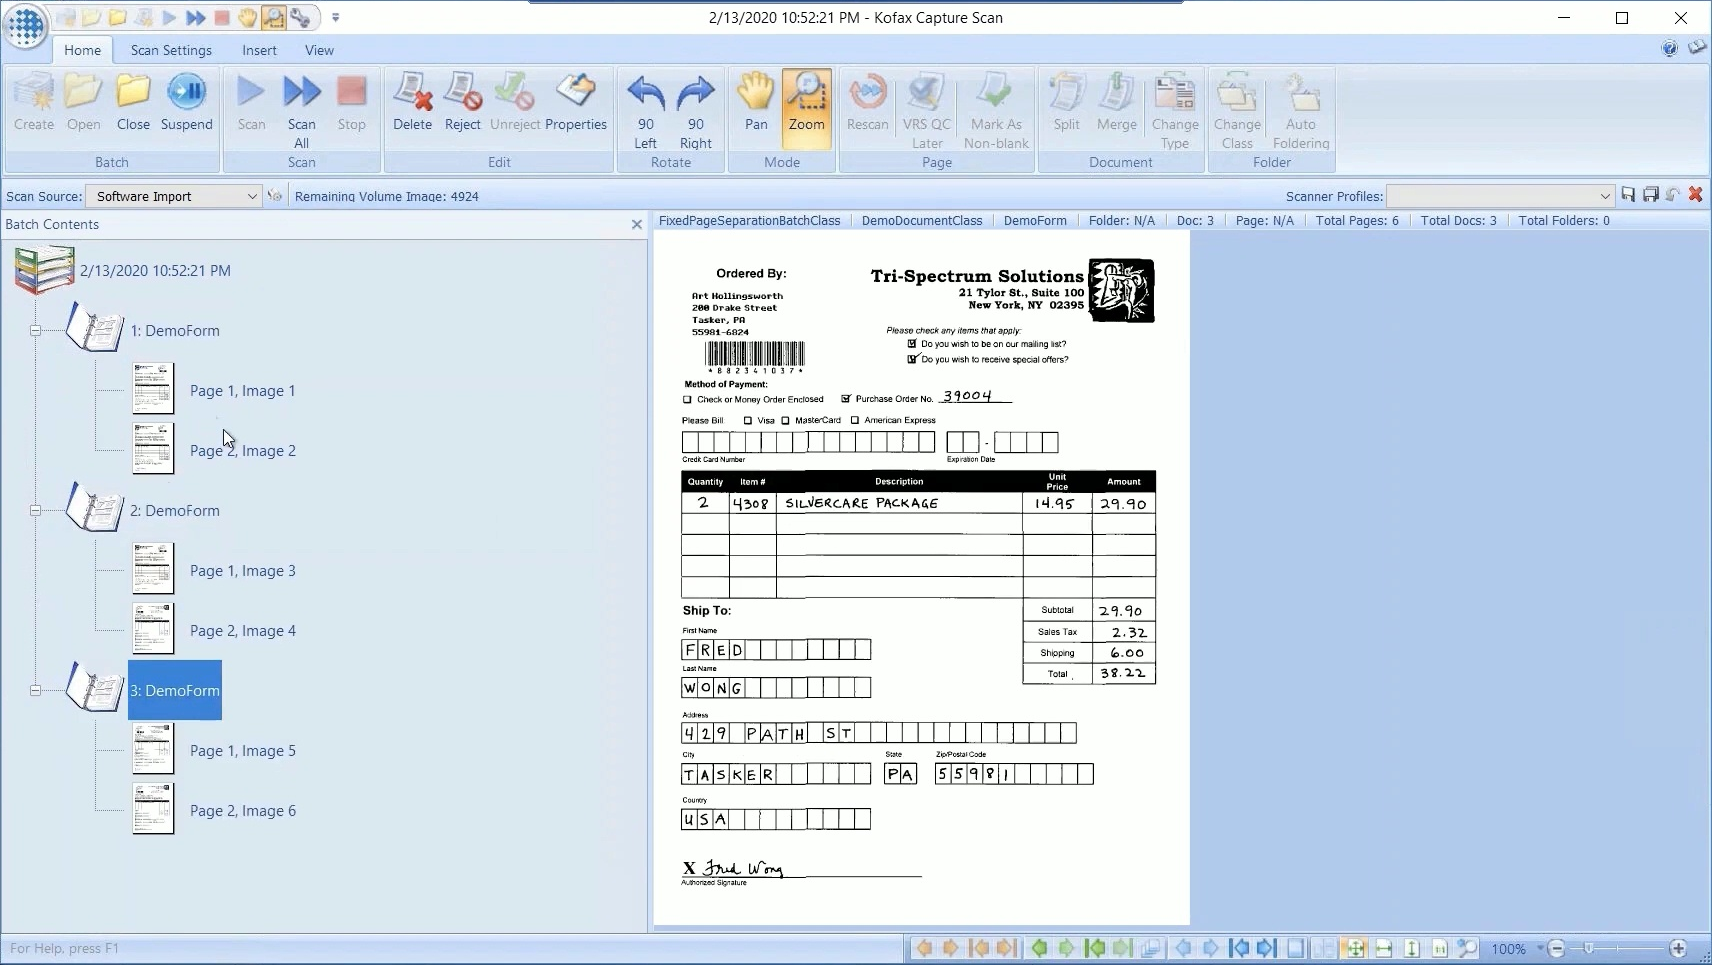
\includegraphics[width=\textwidth]{imaxes/b-estado-arte/kofax-capture}
        \label{fig:hough-punto-imagen}
    \end{subfigure}
    \begin{subfigure}[b]{0.9\textwidth}
        \centering
        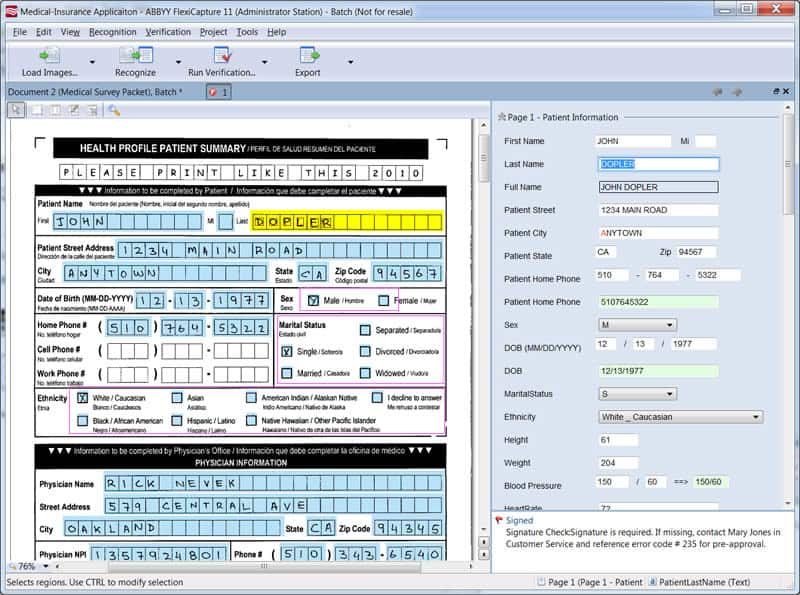
\includegraphics[width=\textwidth]{imaxes/b-estado-arte/abbyy-flexicapture}
        \label{fig:hough-intersection}
    \end{subfigure}
    \caption{Kofax Capture (arriba) y ABBYY FlexiCapture (abajo)}
    \label{fig:kofax-capture-y-abbyy-flexicapture}
\end{figure}

\subsection{Grooper}

Grooper \cite{solucionesComerciales_bisok_grooper} (ver imagen \ref{fig:grooper-bisok}) está hecho por Bisok y a priori parece seguir próxima en características a las dos anteriores. No obstante durante la búsqueda de información ha llamado la atención la mala organización de la información en la web oficial donde no existe una página o documento lineal que explique las características de la aplicación. Una característica destacable es el uso de técnicas de Procesamiento de lenguajes naturales para encontrar párrafos y frases en un documento o ser capaz de distinguir las clausulas en un contrato. También permite seleccionar el engine de \emph{\acrlong{ocr}} utilizado entre un abanico de opciones.

\subsection{Capture de ChronoScan}

Capture de ChronoScan \cite{solucionesComerciales_chronoScanCapture_chronoScanDocumentCapture} (ver imagen \ref{fig:chronoscan-capture}) es una aplicación individual más limitada en funcionalidades que las anteriores. Soporta el flujo normal de lotes con documento pero no dispone de arquitectura cliente servidor por lo cual su uso puede ser más interesante para pequeñas empresas o usuarios individuales. En este sentido la licencia permite su uso sin restricciones siempre que no sea en un contexto profesional.

\subsection{DocAcquire}

DocAcquire \cite{solucionesComerciales_docAcquire_docAcquire} es una solución \emph{\acrlong{saas}} y no dispone de versión de escritorio. Se puede probar de forma gratuita acudiendo a la web oficial. Es la aplicación más simple de todas y, al menos en la versión de prueba, parece que las acciones están bastante limitadas. No se pueden eliminar tipos de documentos una vez creados. Utiliza en engine Tesseract para \acrshort{ocr}.

\subsection{Textract y Document AI}

Dos servicios diferentes a los productos anteriores pero aplicables al problema son, Textract de Amazon \cite{solucionesComerciales_amazon_textract} y Document AI de Google \cite{solucionesComerciales_google_documentAI}. Ninguno de los dos suporta el flujo de información explicado ni están pensados para ser solución para el usuario final. Lo que ofrecen es un \emph{\acrlong{api}} capaz de recibir documentos y generar información estructurada como salida. El caso de Textract es totalmente opaco y por tanto no configurable. La salida consiste en ficheros JSON donde puede haber varios tipos de objetos: páginas, líneas y palabras, información de formularios (pares clave-valor), tablas, y elementos seleccionables como casillas. Además es capaz de identificar notas manuscritas. El servicio de Google permite definir \emph{processors}, que son plantillas específicas para modelos de documentos concretos. Actualmente parece que el servicio es muy reciente y está mayormente en beta. Cualquiera de ellos podría utilizarse para construir una solución más completa. Como otros servicios en la nube, el coste depende de la carga de trabajo procesada.

Después de revisar todas estas alternativas uno de los elementos comunes es el procesado por lotes. En general se deja en manos de los usuarios definir cómo son los modelos de los documentos por medio de un editor que selecciona regiones fijas y les asigna una topología. Estas dos características apuntan a que el sistema.

\begin{figure}
    \centering
    \begin{subfigure}[b]{0.9\textwidth}
        \centering
        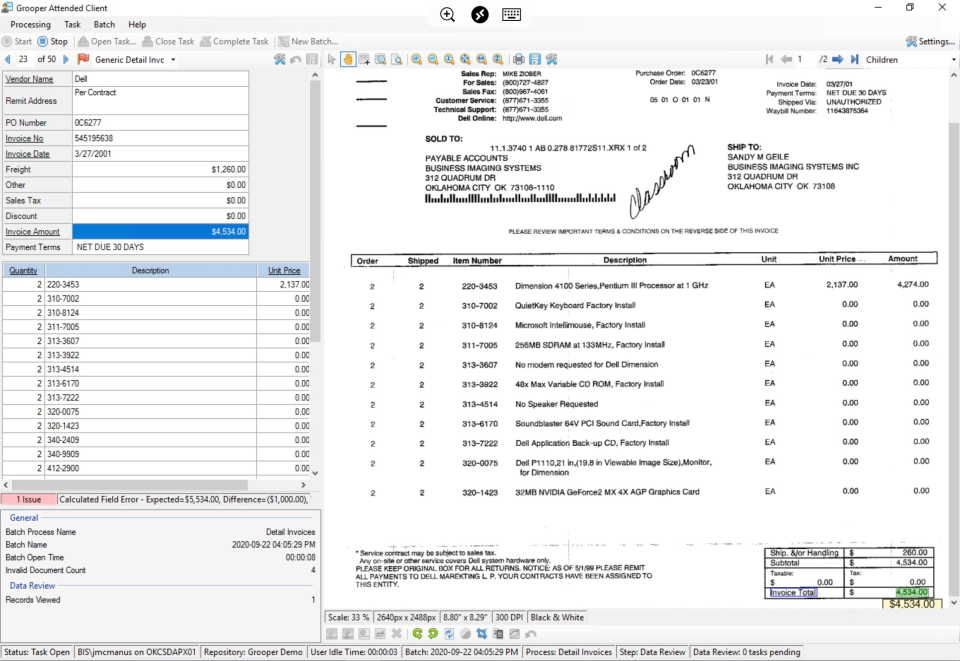
\includegraphics[width=\textwidth]{imaxes/b-estado-arte/bisok-grooper}
        \caption{Grooper, la solución de Bisok}
        \label{fig:grooper-bisok}
    \end{subfigure}
    \begin{subfigure}[b]{0.8\textwidth}
        \centering
        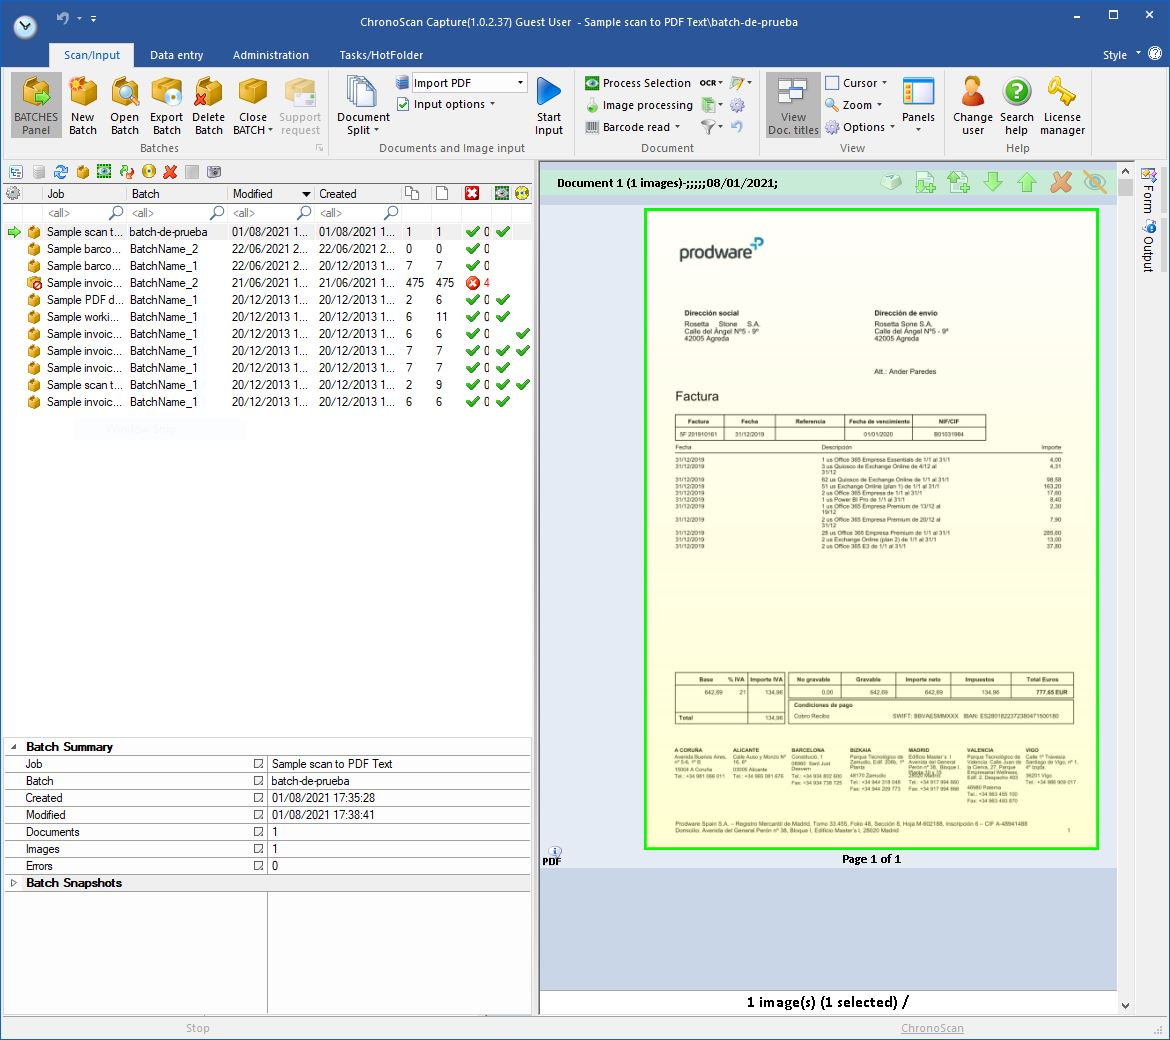
\includegraphics[width=\textwidth]{imaxes/b-estado-arte/chronoscan-capture}
        \caption{ChronoscanCapture con uno de los documentos usando en el proyecto}
        \label{fig:chronoscan-capture}
    \end{subfigure}
%    \caption{Kofax Capture (arriba) y ABBYY FlexiCapture (abajo)}
%    \label{fig:grooper-y-chronoscan-capture}
\end{figure}
 %%%%                          %%%%
%%%% FUNDAMENTOS TECNOLÓGICOS %%%%
%%%%                          %%%%

\chapter{Fundamentos tecnológicos}
\label{chap:fundamentos-tecnologicos}

El objetivo de este capítulo es sentar las bases tecnológicas y teóricas sobre las que se ha llevado a cabo el proyecto.

\section{El formato PDF}

PDF es un formato digital para la creación de documentos introducido por Adobe Systems en 1993 \cite{adobe_systems_inc_quick_2010}. En los siguientes años el uso de este formato se extendió por toda la sociedad tanto en el ámbito público como privado. En el año 2008 la ISO publicó el estándar 32000-1 a partir de la versión 1.7 liberada por Adobe \cite{adobe_systems_inc_iso_2008}. Con posterioridad se publicó la versión 2.0 como ISO 32000-2 \cite{international_organization_for_standardization_iso_2017} en el año 2017 y una actualización en el 2020. PDF es un modelo de representación de imágenes que deriva del lenguaje PostScript para descripción de páginas. El modelo de imagen admite gráficos y texto de forma independiente al dispositivo de salida.

\subsection{Estructura de un PDF}

Un PDF no es un documento de texto, es un fichero binario de 8 bits que posee cierta estructura. El formato soporta varios tipos de datos para la representación de la información. Entre ellos está el formato \verb|String| que se utiliza para representar texto. También hay arrays, diccionarios (tablas asociativas con pares clave/valor) y tipo más básicos como booleanos, enteros o reales. Con estos tipos de datos se construyen objetos que son los que finalmente almacenan la información que se visualiza.

A nivel estructura física, un PDF tiene cuatro regiones. En orden secuencial están, la cabecera, que indica que se trata de un PDF y versión del estándar utilizado. El cuerpo que almacena todos los objetos definidos. Después está la Tabla de Referencias Cruzadas que se utiliza para la navegación y/o avance por el documento. En la tabla están los valores de desplazamiento para todos los objetos indirectos del documento. El cuarto elemento es el \verb|trailer|. Contiene varias claves, las más importantes son \verb|Size| que informa del número de entradas en la Tabla de Referencias Cruzadas y \verb|Root| que apunta al Catálogo del documento, lugar de comienzo de los objetos.

\section{Información de coordenadas en documentos}

La base de este proyecto consiste en utilizar las coordenadas físicas de los textos existentes en los documentos. Dado que los PDF pueden contener una representación textual o simplemente imágenes por cada página, es necesario encontrar una solución aplicable a cada caso y que permita un tratamiento homogéneo en los sucesivos pasos.

\subsection{El microformato HOCR y otras alternativas}


\subsection{Pdftotext e información de bounding box}

\verb|pdftotext| es una herramienta que permite extraer el texto contenido en un PDF. Existen otras herramientas similares, por ejemplo Apache PDFBox \cite{the_apache_software_foundation_apache_nodate}, pero durante el desarrollo \verb|pdftotext| fue la que mostró los resultados más útiles para los objetivos del proyecto. La implementación original de esta utilidad fue realizada por Glyph \& Cog \cite{glyph__cog_llc_glyph_nodate-1} junto con otras herramientas para tratamiento del formato PDF. En el año 2005 nace la librería Poppler a partir del \emph{fork} de la versión 3.0.3 del visor de xpdf \cite{kristian_hogsberg_poppler_2012}. La implementación de Poppler está disponible por defecto en las principales distribuciones Linux. Además del extractor de texto, el proyecto tienen otras utilidades para tratamiento de PDF, por ejemplo, separación y unión de páginas, obtención de imágenes, etc.

La salida con la información de coordenadas, o bounding box, además del texto existe gracias a una aportación al proyecto del año 2010 de Kenneth Berland \cite{kenneth_berland_poppler_2010}. La información se proporciona en formato XHTML y se identifican \emph{tags} para bloques, lineas y palabras. En cada uno se informa de la localización del rectángulo que engloba al elemento con cuatro valores

%% Incluir imagen del rectángulo


\section{OCR con Tesseract}

Existen numerosas herramientas para llevar a cabo Reconocimiento Óptico de Caracteres. Entre ellas destaca Tesseract. Tesseract es un \emph{engine} de código abierto y desarrollado inicialmente por Hewlett Packard entre los años 1985 y 1995. Después de un periodo sin actividad, en el 2006 el proyecto fue recuperado por Google, que lo mantiene desde entonces.

Hoy en día tiene soporte para más de cien idiomas y la red neuronal que utiliza \footnote{Desde la versión 4, Tesseract utiliza una red LSTM. Esta es una red neuronal de tipo recurrente o RNN} puede ser entrenada para casos específicos si fuese necesario. Existe una amplia documentación en la web oficial, además, numerosos tutoriales en la red permiten familiarizarse con la herramienta al tratarse de un proyecto bien conocido y de larga trayectoria.

Se puede obtener como salida el texto reconocido y también la información de las coordenada, sobre el documento, de las palabras detectadas. Esta información resulta fundamental para poder aplicar las plantillas utilizadas este proyecto.

\section{Transformada de Hough}

La transformada de Hough es una técnica de visión por computador utilizada para detectar figuras parametrizables, tales como líneas o círculos. El algoritmo parte de una imagen binaria que representa los bordes encontrados por una detector de bordes. A continuación se calculan todas las posibles líneas que podrían pasar por cada punto y se lleva a cabo una votación. Se seleccionan las líneas más votadas, entre todas las detectadas.

Este algoritmo proporciona una manera automática de localizar los bordes entre líneas de las tablas de muchos documentos y evita la necesidad de incorporar dicha información a las plantillas de forma manual. Se utiliza la implementación incluida en la librería OpenCV.

\section{GNU Make}

GNU Make es una herramienta que permite automatizar transformaciones sobre ficheros. \verb|make| es capaz de construir ejecutables a partir del código fuente de un proyecto. Para ello utiliza un fichero \verb|makefile| que contiene todas las reglas necesarias.

\section{Flex y Bison}

Flex y Bison son dos herramientas utilizadas en conjunto para construir analizadores sintácticos. ¿Qué es un analizador sintáctico?

La primera se utiliza para crear escáneres y la segunda para generar parsers. Ambas utilizan como entrada unos ficheros que definen las reglas válidas.

\section{Ansible}



\section{Docker}




%% Valorar si mencionar otras herramientas como:
% Extracción de texto: , pdftotext
% Pretty print de JSON: jq

 %%%%             %%%%
%%%% METODOLOGÍA %%%%
%%%%             %%%%

% TODO explicar cómo facilita Scrum la adaptación para la construcción del prototipo web

\chapter{Metodología}
\label{chap:metodologia}

\lettrine{E}{n} este capítulo trata sobre metodologías aplicadas a proyectos de software y en particular la metodología seleccionanda para el este trabajo, Scrum.

Las metodologías para que se refieren al Ciclo de Vida del Desarrollo de Software, SDLC en inglés, son procesos y prácticas utilizadas por los equipos de desarrollo de software para tratar con éxito el SDLC.

Históricamente la metodología más conocida es la metodología de desarrollo en Cascada que tiene su origen en un artículo científico de Winston W. Royce en los años 70. Esta metodología se completa en cinco etapas:

\begin{enumerate}
    \item Análisis de requisitos
    \item Diseño
    \item Implementación
    \item Verificación
    \item Mantenimiento
\end{enumerate}

Un proyecto se realiza en un único ciclo,  las etapas se ejecutan en orden y sin solapamientos. Este es un modelo que resulta rígido e impone muchas limitaciones: las pruebas de integración no se pueden llevar a cabo hasta completar todo el desarrollo, los usuario no puede probar la aplicación hasta el final del proyecto, que se puede demorar meses o incluso años. En este modelo no hay oportunidad para que los cliente u otras partes interesadas puedan ofrecer sus opiniones.

Para tratar de ofrecer una alternativa a las limitaciones impuestas por el desarrollo en cascada, fueron propuestas otras metodologías, como la metodología en espiral o la metodología en V. Pero no fue hasta mediados de los años 90 que no aparecen las primeras tecnologías ágiles. Especialmente en el año 2001 se publicó el Manifiesto por el desarrollo ágil que valora los siguientes cuatro puntos:

\begin{itemize}
    \item Individuos e interacciones sobre procesos y herramientas.
    \item Software funcionando sobre documentación extensiva.
    \item Colaboración con el cliente sobre negociación contractual.
    \item Respuesta ante el cambio sobre seguir un plan.
\end{itemize}

En este proyecto se utiliza Scrum que pertenece al conjunto de metodologías ágiles.

\section{Scrum}

\emph{The Scrum Guide} es la guía oficial donde se presenta el framework Scrum. Scrum es un marco de trabajo para ayudar en la creación de valor mediante soluciones adaptativas a problemas complejos. Scrum propone una filosofía general, varios roles para las tareas, unos eventos que se repiten de forma cíclica y unos artefactos como producto del trabajo.

Scrum no está limitado a proyectos de software. Siempre y cuando se respeten sus características, se posiciona como un modelo más general, que se puede aplicar a cualquier proyecto donde sea capaz de aportar valor.

\subsection{Roles}

La unidad de trabajo está formada por el Equipo Scrum. Se consideran tres roles dentro del Equipo:

\begin{itemize}
    \item Los \textbf{Desarrolladores} son todas las personas que contribuyen a crear los incrementos durante cada ciclo. Las cualidades de las personas consideradas desarrolladoras pueden ser variadas. Los desarrolladores son responsables del mantenimiento del Sprint Backlog.
    \item El \textbf{Product Owner} es la persona responsable de maximizar el valor resultante del trabajo del Equipo Scrum. El framework no indica como debe conseguir este objetivo. El Product Owner también es responsable del Product Backlog.
    \item El \textbf{Scrum Master} es responsable de asegurar que se siguen los principios del marco de trabajo y entre sus obligaciones está la de actuar apoyando a los demás miembros del equipo para la mejora de las prácticas relacionadas con Scrum. De forma general es responsable de la efectividad del Equipo.
\end{itemize}

\subsection{Eventos}

El ciclo de vida de Scrum está contenido en el Sprint. Durante un Sprint se lleva a cabo el trabajo generador de valor para el proyecto. La duración de un Sprint es flexible pero debería estar entre una y cuatro semanas. Debe ser lo suficientemente largo como para dar tiempo a la realización de trabajo significativo, pero no tan largo que se pierda de vista el objetivo del propio Sprint, o que el objetivo planificado cambie y ya no sea válido. Dentro del Sprint se suceden los otros cuatro tipos de eventos.

\begin{figure}[hp!]
    \centering
    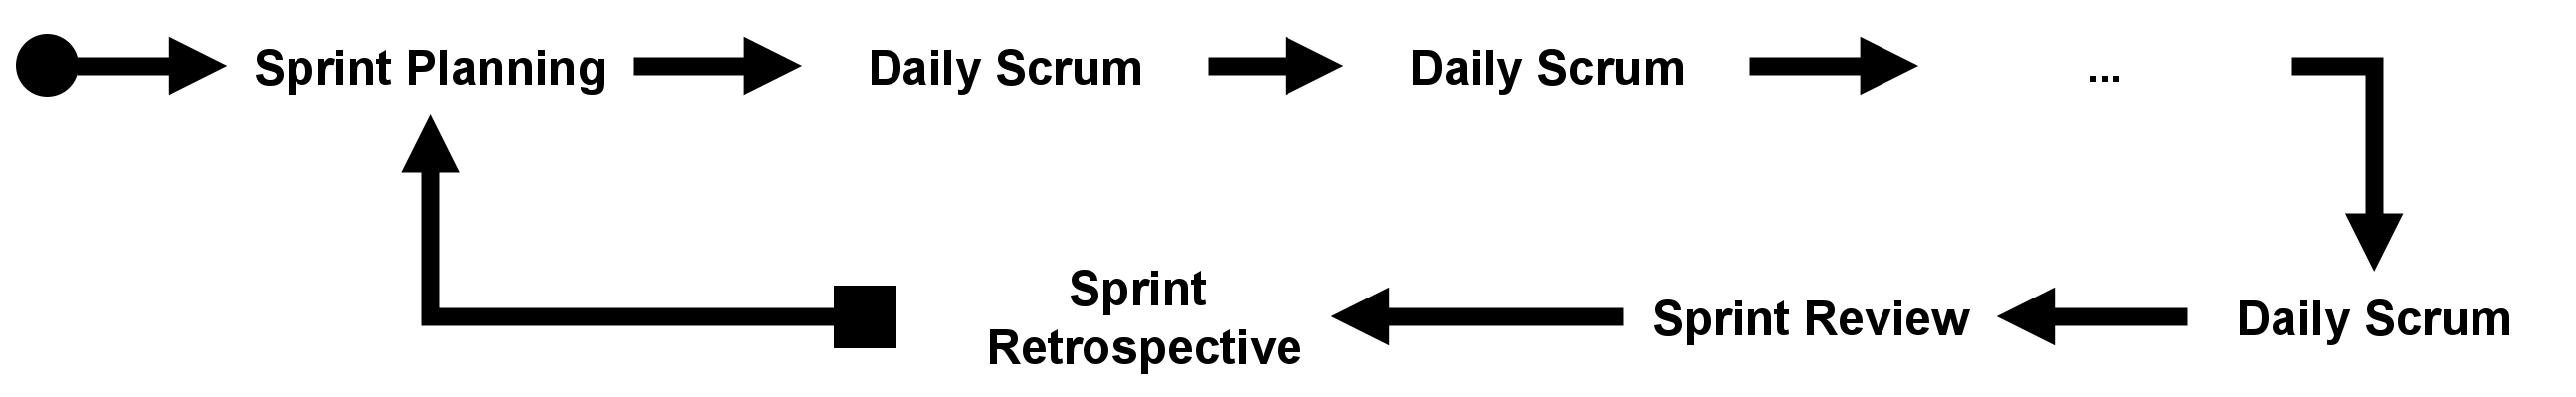
\includegraphics[width=1.0\textwidth]{imaxes/d-metodologia/ciclo-scrum.png}
    \caption{Ciclo de vida de Scrum.}
    \label{fig:ciclo-vida-scrum}
\end{figure}

\begin{itemize}
    \item El \textbf{Sprint Planning} es da comienzo a un nuevo Sprint. En este evento se acuerda el trabajo que se va a realizar durante el Sprint. El equipo completo trabaja para establecer las tareas particulares que serán abordadas en el periodo. En el Sprint Planning pueden participar otras personas involucradas con el proyecto pero que no pertenezcan al Equipo. Su ayuda puede ser necesaria para aclarar aspectos de las tareas o los objetivos.
    En este evento es importante dar respuesta a cómo se puede añadir más valor al producto. El Objetivo del Sprint debe quedar claramente definido y para ello todo el equipo colabora. También hay que establecer qué cosas se pueden llevar a cabo durante el Sprint. Se seleccionan por tanto todas aquellas tareas que deberán ser abordadas. Por último se requiere decidir cómo se llevarán a cabo las tareas. Puede ser necesario conseguir un mayor refinamiento para que los Desarrolladores puedan tomar las decisiones correspondientes.

    \item El \textbf{Daily Scrum} es un evento de 15 minutos para revisar el avance hacia el objetivo del Sprint. Como en otros aspectos de Scrum, el framework no explicita la técnica o estructura de la reunión, pero insiste en que es el momento de comunicar dificultades, logros y planificar el trabajo para la jornada siguiente. A esta reunión solo acuden los Desarrolladores.
    
    \item El \textbf{Sprint Review} tiene por objetivo analizar y enseñar las mejoras alcanzadas durante el Sprint. A esta reunión acudirá no solo el Equipo sino también todas las personas involucradas de forma amplia. Esta sesión no solo es de exposición, también sirve para decidir futuras adaptaciones. De hecho Scrum propone este momento para seleccionar que es lo próximo a completar.
    
    \item El \textbf{Sprint Retrospective} se propone como una reunión para mejorar la calidad y la efectividad. Esta es una oportunidad para revisar todos los componentes del proceso de trabajo y encontrar problemas en procesos, herramientas, comunicaciones, etc. La reunión debe responder a qué sosas fueron bien, cuales fueron mal y como se gestionaron. Se deben proponer acciones de mejora para los problemas. Si es oportuno, estas acciones podrían se incluidas en el Sprint Backlog.
\end{itemize}

\subsection{Scrum Artifacts}

Los Artefacto son la representación del trabajo o del valor. Cada uno de los artefactos está relacionado con un compromiso en el proyecto.

\begin{itemize}
    \item El \textbf{Producto Backlog} el la lista priorizada de todo aquello que debe realizarse para mejorar el producto. Es la fuente de trabajo utilizada por el Equipo. Todos los elementos que quepan dentro de un Sprint son susceptibles de ser incorporados al Sprint Backlog.
    \item El \textbf{Sprint Backlog} cotiene el Objetivo del Sprint, un subconjunto del trabajo exisnte en el Project Backlog y que será el trabajo acometido durante el Sprint. Por último contendrá un plan de trabajo para conseguir aportar el valor al proyecto.
    \item Los \textbf{Incrementos} son las unidades que hacen avanzar hacia en Objetivo del Proyecto. Puede ser cualquier cosa siempre y cuando se comporte de manera aditiva a todos los demás Incrementos y sea utilizable. Los incrementos deben funcionar de forma conjunta, así que serán revisados con el objetivo de comprobar su calidad.
\end{itemize}

De forma general Scrum es un proceso en cuatro etapas:

\begin{enumerate}
    \item El Product Owner toma un problema complejo y lo transforma en unidades individuales de trabajo.
    \item El Equipo Scrum realiza una selección del trabajo y lo transforma en un Incremento de valor durante un Sprint.
    \item El Equipo y otras partes interesadas revisar los resultados y ajustan todo lo necesario para el siguiente Sprint.
    \item Volver a empezar.
\end{enumerate}

\section{Uso de Scrum en el proyecto}
\label{sec:uso-scrum-en-el-proyecto}

Para la aplicación del Scrum a proyecto han sido necesarias algunas adaptaciones por la propia naturaleza del TFG. El rol de Product Owner lo ha realizado el director del proyecto. El Equipo de Desarrollo está formado únicamente por el alumno, que también ha hecho las funciones de Scrum Master.

Las reuniones se han reducido al no existir otras personas con las cuales coordinarse. Se han mantenido las reuniones con el director del proyecto para la revisión del Sprint y el Sprint Planning. Las reuniones se han llevado a cabo de forma telemática.

Se ha recurrido al concepto de Spike para la adquisición de conocimiento. Un Spike es una historia de usuario especialmente indicada para dar tiempo al equipo a explorar una tecnología desconocida, comprender una implementación con la que no se está familiarizado, elaboración de prototipos.

\section{Herramientas de apoyo a la metodología}

Para organizar las historias de usuario y poder dividir el trabajo en tareas se ha recurrido al servicio web Github \footnote{\url{https://github.com/}}. Asociado a cada repositorio de código se pueden crear tableros para organizar el trabajo.

La herramienta permite dividir el espacio de trabajo en columnas que representan historias de usuario. También se creó una columna para representar el trabajo en curso y tantas colunas como sprints para ir colocando las tareas realizadas.

También se recurrió a Microsoft Project 2013 que si bien no resulta tan cómodo como el tablero de Github para desgranar el detalle de las tareas, si que proporciona una visión más general del avance del proyecto y permite hacer su seguimiento.

 %%%%                       %%%%
%%%% ENTORNO DE DESARROLLO %%%%
%%%%                       %%%%

\chapter{Entorno de desarrollo}
\label{chap:entorno-desarrollo}

\lettrine{E}n este capítulo se explica como es el entorno utilizado para llevar a cabo el proyecto. En particular se comentan las herramientas específicas y las tecnologías utilizadas.

\section{Útiles de trabajo}

La máquina de trabajo consistió en un portátil HP con un procesador Intel i5 de segunda generación, 12 GB de RAM y sistema operativo Ubuntu. Para el desarrollo en Python se utilizó Eclipse con el plugin Pydev
\footnote{https://www.pydev.org}. Los editores Atom y vim sirvieron para los scripts y el código en C de los escáneres y parsers. La memoria en \LaTeX está elaborada con TeXstudio. Se utilizó Zotero para las referencias y el plugin Better BibTeX (BBT) 
\footnote{https://retorque.re/zotero-better-bibtex} para gestionar las claves de la bibliografía. Los diagramas están hechos con yEd, la herramienta para creación de diagramas de yWorks 
\footnote{https://www.yworks.com/products/yed}. El control de versiones se llevó a cabo con git y Github. Dropbox Paper tiene la facilidad de representar notación Markdown con un diseño agradable así que fue utilizado para la organización, borradores, notas, etc.

\section{Tecnologías}

\subsection{OpenCV}

\subsection{Flex}

\subsection{Bison}

\subsection{Docker}

\subsection{Ansible}


 %%%%            %%%%
%%%% MATERIALES %%%%
%%%%            %%%%

\chapter{Materiales}
\label{chap:materiales}

Análisis de los documentos utilizados para el desarrollo del proyecto. Modelos PDF de texto facilitados por Betmedia. Modelos PDF imagen facilitados por Solco.

Caracterización de las regiones de interés.

Datos para identificar los documentos. En este caso, NIF, CIF.

 %%%%                %%%%
%%%% IMPLEMENTACIÓN %%%%
%%%%                %%%%

\chapter{Implementación}
\label{chap:implemetación}

\section{Plantillas y regiones}
\subsection{Información contenida en las plantillas}
\subsection{Tipos de regiones}

\section{Generación de lenguaje intermedio}
\subsection{Información de bounding box}
\subsection{Concepto de líneas e identificación}
\subsection{Selección de palabras}
\subsection{Uso de la transformada de Hough}

\section{Generación de lenguaje estructurado}
\subsection{Selección dinámica de escáner y parser}
\subsection{Ventajas como modelo de producto???}

\section{Mecanización del proceso}
\subsection{Motor / engine}
\subsection{Estructura de directorios}
\subsection{Flujo de información}

\section{Compilación y despliegue}
\subsection{Makefile}
\subsection{Ansible y Docker}


Este capítulo describe el diseño y la implementación de la solución construida.

%% La implementación está diseñada para recibir peticiones de conversión y generar la salida correspondiente en formato estructurado. El número de ficheros que se pueden tratar en cada ejecución solo está limitado por las capacidades del sistema de ficheros o del SO donde se ejecute. Cada invocación produce una tarea en el sistema, que se gestiona de forma individual. Una vez que se reciben los ficheros para su tratamiento, se crea una ruta específica para ese trabajo y comienza el proceso. En %% cada etapa se crean nuevos ficheros intermedios que, según se verá más adelante, se mueven a destinos designados para cada paso. Los documentos se tratan página a página. El motor encargado de conducir el flujo de información está implementado en lenguaje Bash. Este \emph{engine} se apoya en varias herramientas adicionales, disponibles en cualquier distribución Linux. Por último, se complementa con el generador de código intermedio y los \emph{parsers} para cada modelo de documento.
%% 
%% % Existen, por tanto, tres partes que se detallarán en las siguientes páginas:
%% 
%% %% \begin{itemize}
%% %%     \item Un motor o \emph{engine} creado con \emph{scripts} en lenguaje Bash. Su cometido es recepcionar los ficheros y transformarlos paso a paso hasta la obtención de la salida final.
%% %%     \item Una aplicación Python encargada de generar el lenguaje intermedio que va a ser procesado.
%% %%     \item Una familia de escáners y parsers desarrollados empleando Flex \cite{estes_flex_2021} y GNU Bison \cite{free_software_foundation_inc_bison_nodate}. Toman como entrada el lenguaje intermedio y lo traducen a un formato estructurado.
%% %% \end{itemize}
%% 
%% %% Se describen a continuación cada una de ellas.
%% 
%% %% \section{El engine}
%% %% La herramienta se planteó como un software que pudiera ser capaz de recibir uno o varios ficheros en cada invocación. Una vez recibido, cada entrada debía ser clasificada e identificada para su correcto tratamiento. Dado que la entrada y la salida serían ficheros, resultaba natural utilizar un lenguaje de programación con facilidades para la manipulación de ficheros. Por ser el entorno de operación y desarrollo un sistema GNU/Linux, se optó por emplear el intérprete de \emph{shell} Bash.
%% 
%% %% Por tratarse de un conjunto de \emph{scripts}, este \emph{pipeline} es flexible tanto para añadir nuevos pasos como para quitarlos. La razón para hacerlo de este modo radica en posibilitar la incorporación de nuevas técnicas de procesado de cualquiera área relevante, como el tratamiento de imagen o la extracción de texto. Cada \emph{script} es independiente y puede ser ser activado o desactivado fácilmente.
%% 
%% %% Convenio de nombrado para evitar perder información o mezclar páginas
%% 
%% %% Elaboración de las plantillas: Las plantillas son ficheros en formato JSON. Contienen las coordenadas de la geometría para las regiones de interés.
%% 
%% %% Generación del lenguaje intermedio: el sistema de generación de lenguaje intermedio debía ser necesariamente flexible. Para poder aplicar técnicas distintas. Se optó por utilizar Python, que tiene mucho soporte y una gran colección de librerías disponibles.
%% 
%% %% Detección de subregiones: Se diseñó un algoritmo sencillo pero eficaz para decidir si una región era subregión de otra dada.
%% 
%% %% Aproximación para la identificación de las líneas individuales: Esta aproximación se basó en intentar caracterizar las líneas mediante propiedades sencillas. La aproximación no dio resultado.
%% 
%% %% Mejora de tiempos: Inicialmente se utilizada el tipo de dato Set y sus operaciones para comprobar la inclusión de unas regiones en otras. Esta aproximación, aunque funcional, no resultaba rápida para su ejecución durante el desarrollo. Se realizó una mejora que comprueba las propiedades geométricas en lugar de basarse en lógica de conjuntos.
%% 
%% %% Obtención de información estructurada
%% %%%% Flex
%% %%%% Bison
%% 
%% %% Despliegue de la aplicación
%% 
%% %% Cambios para integrarse con la GUI
%% %%%% Exponiendo las coordenadas 
%% %%%% Uso de Docker
%% 
%% \section{Estructura física}
%% 
%% Para entender más fácilmente las características de la implementación se describen primero la estructura de directorios que conforman el proyecto. 
%% La estructura y funcionalidad de los directorios del proyecto es importante para entender como se trata la entrada. Esta estructura general se puede consultar gráficamente en XXX. La aplicación se compila y distribuye por medio de un \verb|Makefile|. También existe un fichero \verb|Dockerfile| configurado para generar la correspondiente imagen Docker del programa. Los principales directorios utilizados son:
%% 
%% \begin{itemize}
%%     \item \verb|conf|, empleado para las configuraciones del \emph{engine}, también la configuración de Tesseract y los datos de entrenamiento.
%%     \item \verb|data| contiene información de los modelos soportados. Principalmente, los identificadores utilizados para reconocer los documentos y las plantillas que relacionan las regiones seleccionadas.
%%     \item \verb|doc| está dedicado a la documentación del proyecto. También contiene todos los ejemplos de ficheros PDF utilizados. Esta memoria, escrita con el sistema de composición de textos \LaTeX,  tiene un repositorio de código propio.
%%     \item \verb|engine| tiene como finalidad alojar todos los \emph{scripts} del \emph{engine}.
%%     \item \verb|input| no está en el repositorio, sino que se crea bajo demanda. Es la ruta base para la entrada de datos consumidos por la aplicación. El nombre puede cambiarse definiendo otro en la configuración del \emph{engine}.
%%     \item \verb|script| mantiene varios \emph{scripts} auxiliares utilizados principalmente para facilitar las ejecuciones durante el desarrollo.
%%     \item \verb|tool-gen-language| es la carpeta dedicada a los fuentes de la herramienta de generación de lenguaje intermedio.
%%     \item Por último, \verb|tool-parser| contiene la aplicación Flex/Bison y los \verb|plugins| que convierten el lenguaje intermedio a la salida JSON.
%% \end{itemize}
%% 
%% \section{Tratamiento inicial de la entrada}
%% 
%% La herramienta es un software \verb|backend|, no está pensada para que un usuario realice las ejecuciones de la aplicación manualmente. Por ello, y aunque no se desarrolló un API para acompañar la solución, si que se definieron varias características con la finalidad de facilitar la depuración durante el desarrollo y servir de primera aproximación para una futura integración en un sistema basado en un diseño por capas.
%% 
%% Cada ejecución se realiza en un directorio propio donde se almacena la entrada, se realiza el tratamiento y se ubica la salida. Además, se facilita al programa invocador un identificador que debe utilizar para la recuperación de los resultados. La ruta al directorio que contiene todas las carpetas de todas las ejecuciones el es directorio \verb|input|, mencionado anteriormente.
%% 
%% Para evitar colisiones en las rutas de trabajo entre distintas ejecuciones, se obtiene una marca de tiempo del instante de recepción de la petición y se utiliza como directorio raíz para el nuevo trabajo. Este \emph{timestamp} se obtiene con el comando \verb|date| configurado para generar un entero de tamaño 16 con la hora UTC del sistema:
%% 
%% \begin{minted}{shell-session}
%% diego@CompaqCQ57:galiasdoc$ date -u +"%s%6N"
%% 1616623143141490
%% diego@CompaqCQ57:galiasdoc$
%% \end{minted}
%% %% TODO centrar y añadir caption: ejemplo de directorio de trabajo
%% 
%% A continuación, se presenta la secuencia de pasos que conforman el comienzo de un trabajo. La primera acción ocurre cuando el invocador ejecuta el \emph{script} \verb|get-job-id.sh|. Este crea el nuevo directorio para el trabajo y todos los directorios internos. Se devuelve el identificador de trabajo al programa llamador.
%% 
%% En este momento el llamador debe copiar el fichero de entrada en la ruta \verb|job_id/frontend|. Por último, se inicia la ejecución cuando se llama al \emph{script} \verb|run.sh|. Se le debe indicar al motor el identificador del \emph{job} que que se quiere iniciar. Para ello, el \verb|job_id| se pasa como parámetro. Los pasos se pueden seguir visualmente en la figura \ref{fig:inicio-aplicacion}.
%% 
%% A partir de este momento el sistema comienza a trabajar. Cada acción llevada a cabo se indica con un mensaje por la salida estándar de la consola. Cuando finaliza, se notifica con otra marca de tiempo del momento final en la ruta \verb|input/job_id/done-<timestamp>|.
%% 
%% \begin{figure}[hp!]
%%   \centering
%%   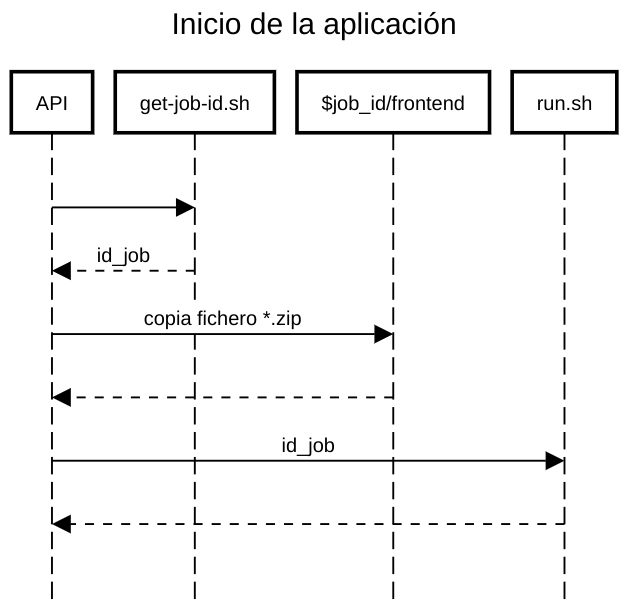
\includegraphics[width=11cm]{imaxes/inicio-aplicacion.png}
%%   \caption{Secuencia de inicio de la aplicación}
%%   \label{fig:inicio-aplicacion}
%% \end{figure}
%% 
%% %% Cambiar diagrama con flecha saliente para indicar que se ejecutan los pasos del engine
%% %% Cambiar "copia fichero *.zip" por "datos entrada"
%% %% La línea de finalización debe devolver el evento de finalización
%% 
%% \section{Flujo de información en el \emph{engine}}
%% 
%% Cuando se invoca el \emph{script} \verb|run.sh| se realizan en secuencia todos los pasos que acaban generado la salida en formato estructurado.
%% 
%% %% Considerar borrado:
%% 
%% %% Primero se descomprimen los datos de entrada y se renombran los ficheros recibidos para que su tratamiento sea seguro al construir las rutas. Seguidamente se realiza una primera extracción de texto con \emph{pdftotext}. En tercer lugar, se realiza una clasificación de los casos basados en texto y aquellos basados en imagen. También se generan imágenes de todas las páginas de los documentos basados en texto. A continuación ya se realiza el Reconocimiento Óptico de Caracteres para los casos %% basados en imagen. Con el OCR completado se trata de identificar cada documento. Lo siguiente es generar el lenguaje intermedio e invocar al \emph{parser} necesario. Por último, se publican los resultados en el directorio de salida del trabajo.
%% 
%% %&
%% 
%% Para facilitar la comunicación, se asume que la entrada llega como un único fichero comprimido. En este primer paso es necesario extraer los contenidos de dicho fichero. Se realiza además un renombrado de cada uno, para evitar errores debidos a caracteres poco amigables con el intérprete de comandos, a la hora de componer las rutas.
%% 
%% Una vez los ficheros PDF ya están disponibles, se realiza una primera extracción de texto con la herramienta \verb|pdftotext|. El objetivo es realizar la clasificación que separe los ficheros de texto de aquellos cuyas páginas son imágenes.
%% 
%% Cuando \verb|pdftotext| en invocado en un PDF sin texto, genera igualmente un fichero de salida cuyo único contenido es un símbolo de fin de página. Por defecto utiliza el carácter \verb|Form Feed| o \verb|0x0D|. Aquellas páginas que dan como resultado únicamente este carácter son movidas al directorio para el tratamiento por imagen, \verb|based-image|.
%% 
%% El siguiente paso consiste en obtener la descripción de las coordenadas de las palabras y las líneas. Para ello \verb|pdftotext| vuelve a ser clave ya que con el flag \verb|-bbox-layout| permite generar un fichero XML que contiene estos datos y también el texto encontrado. Respecto a la calidad del texto hay que tener presente que muchos PDF introducen variaciones en las palabras, típicamente añadiendo espacios entre las letras. Estos problemas son tratados posteriormente.
%% 
%% A continuación se muestra un fragmento de una de estas salidas XML:
%% 
%% \begin{minted}[linenos]{xml}
%% <head>
%% <title>Factura ES1864857 - OVH</title>
%% </head>
%% <body>
%% <doc>
%%   <page width="595.000000" height="842.000000">
%%     <flow>
%%       <block xMin="1223.064810" yMin="168.431792" xMax="1353.159365" 
%%           yMax="203.373692">
%%         <line xMin="1223.064810" yMin="168.431792" xMax="1353.159365" yMax="203.373692">
%%           <word xMin="1223.064810" yMin="168.431792" xMax="1353.159365" 
%%               yMax="203.373692">Factura:</word>
%%         </line>
%%       </block>
%%     </flow>
%%   </page>
%% </doc>
%% </body>
%% </html>
%% \end{minted}
%% 
%% %% XXX Explicación de representación en coordenadas
%% 
%% Para facilitar a la aplicación gráfica la visualización de los contenidos detectados surgió la necesidad de proporcionar imágenes de las páginas de los documentos de tipo texto. Esto se realiza invocando a la herramienta \verb|pdftocairo|. 
%% 
%% La siguiente fase se extraen contenidos y coordenadas de las páginas con imágenes. En este caso se utiliza Tesseract. Además del fichero de entrenamiento estándar está disponible otro de mayor tamaño y que resulta más certero con un coste temporal mayor. Para los casos tratados los resultados con la versión estándar fueron suficientemente satisfactorios. Todos los ficheros de entrenamiento de la aplicación están disponibles en la web oficial del proyecto XXX. Existe además la posibilidad de %% crear ficheros de entrenamiento propios para casos específicos, el proceso también está documentado en la web oficial XXX. La salida de Tesseract que se utiliza no es simplemente el texto reconocido. Al igual que en el caso de las páginas con texto se necesitan las coordenadas de los elementos encontrados. Esto se consigue con el parámetro \verb|tessedit_create_hocr|. La salida en este caso será un fichero en formato HOCR.
%% 
%% %% XXX Imagen del fichero HOCR abierto con alguna aplicación de visualización
%% 
%% Para poder aplicar la plantilla a un fichero correcta a un fichero determinado es necesario realizar un emparejamiento. En este caso se optó por buscar en los documentos datos específicos que no causaran colisión con otros documentos. Dado que los datos disponibles son facturas de empresas, se optó por utilizar los códigos NIF o DNI del emisor en este caso y que por ley son obligatorios en este tipo de documentos XXX. Se creó un registro con estos códigos y se realiza una búsqueda con %% \verb|grep| sobre los textos extraídos bien con Tesseract bien con \verb|pdftotext|. En los casos tratados esta búsqueda fue lo suficiente robusta.
%% Cuando un patrón es encontrado, se crea en el directorio donde se está tratando el documento un fichero con el nombre dado al documento en la fase de renombrado y cuyo contenido es el propio identificador encontrado.
%% 
%% \begin{minted}{shell-session}
%% diego@CompaqCQ57:galiasdoc$ ls input/1617643045714091/based-text/2/*id
%% input/1617643045714091/based-text/2/2.id
%% diego@CompaqCQ57:galiasdoc$ cat input/1617643045714091/based-text/2/*id
%% B83834747
%% \end{minted}
%% 
%% Llegados a este punto ya está disponible toda la información necesaria para construir la salida. Hay dos \emph{scripts} más que se ejecutan. Primero se invoca a la herramienta de generación de lenguaje intermedio y después al parser Bison correspondiente. El último \emph{script} mueve los resultados al directorio de salida del \emph{job}, donde podrán ser recuperados. Además se crea en la raíz del \emph{job} un fichero vacío cuyo nombre es el \emph{timestamp} del momento finalización de de la %% ejecución.
%% 
%% \section{Generación del lenguaje intermedio}
%% 
%% \subsection{Definiendo regiones con plantillas}
%% 
%% Las plantillas son documentos JSON que contienen toda la información necesaria para localizar el texto de interés del documento. La creación de las plantillas se ha realizado manualmente. En estas plantillas se definen áreas cuadradas o rectangulares donde están las palabras que se desea generar en formato estructurado. Se distinguen cuatro tipos de regiones.
%% 
%% La más sencilla es una región de tipo secuencia, esto es, los contenidos se ordenarán de izquierda a derecha y de arriba a abajo. Después están las tablas simples que contienen una única columna y múltiples filas o viceversa. El último tipo de región son las tablas de datos con nxm filas y columnas. En el interior de cada subregión el texto se ordena siguiendo el mismo procedimiento que en el caso más básico.
%% 
%% %% Para ampliar: más tipos de informaciones recogidos en las plantillas
%% 
%% \subsection{Estructurando la información}
%% 
%% El cometido principal de la herramienta de generación de código intermedio es transformar el texto extraído en un lenguaje con elementos gramaticales que permitan tratarlo con un parser. A partir de las regiones definidas en las plantillas y las coordenadas de las palabras se hace un filtrado. Se descartan todas las palabras que no encajen en ninguna región, las demás se asocian a la región a la que pertenezcan.
%% 
%% Los elementos principales del programa se detallan a continuación:
%% 
%% Primero se tratan los argumentos de entrada. Especialmente se selecciona XXX ¿qué cosas se seleccionan? XXX
%% Después se realiza el parse de los datos de entrada. Esto transforma la información de coordenadas y los valores de las palabras en estructuras en memoria. Datos que ambos orígenes de datos comparten el formato HTML, es posible utilizar el parser por defecto que proporciona Python, la clase \verb|HTMLParser|, con la finalidad de extraer las líneas y palabras proporcionadas. Se crearon dos clases que especializan la anterior, \verb|xmlTMLParser| y \verb|hocrHTMLParser| para las particularidades %% de cada tipo de origen.
%% 
%% En la aplicación existen tres conceptos distintos de lo que es una línea. La idea más inmediata de una línea es aquella que se aprecia visualmente sobre un documento. Estas son las líneas que querríamos que el sistema identificara como tales. XXX extender concepto de línea con las otras dos ideas. Creo recordar: la línea área que encaja dentro de una columna, pero no se extiende a otras. XXX. Un problema encontrado en esa asignación de palabras a líneas es que hay casos donde una línea abarca %% más de una columna. Para generar correctamente el lenguaje, cada palabra debe pertenecer a una única línea y la línea debe pertenecer a una única columna. Se realiza por tanto un troceado de las líneas excesivamente extensas. Se fraccionan y se asignan a las regiones que les corresponden.
%% 
%% En este punto ya se ha preparado la información para poder llevar a cabo el tratamiento. Se crea en un objeto tipo diccionario que contiene todos los datos conocidos hasta ahora:
%% 
%% \begin{itemize}
%% 	\item Las líneas,
%% 	\item las palabras,
%% 	\item las regiones definidas en las plantillas,
%% 	\item el número de página actual,
%% 	\item el número de páginas que contiene el documento completo,
%% 	\item la ruta a la imagen de la página actual.
%% \end{itemize}
%% 
%% La penúltima fase asigna contenidos a las regiones definidas en las plantillas y por último se escriben todos los resultados a disco.
%% 
%% \subsection{Tratamiento de las líneas y las regiones}
%% 
%% El objetivo principal en esta fase es asociar a cada región las líneas que le corresponden. Primero se realiza una clasificación de las regiones según apliquen a una única página, por ejemplo la primera o la última; a múltiples páginas o a todas las páginas del documento. Lo que se hace es escoger las regiones que aplican a la página actual atendiendo al número de página que tiene y su posición dentro del documento. Además de los casos básicos mencionados anteriormente, para el correcto %% tratamiento fue necesario implementar comportamientos para las siguientes categorías: 
%% 
%% \begin{itemize}
%% 	\item R1: una región formada por una columna de cabeceras a la izquierda
%% 	\item R2: región con cabecera en la fila superior
%% 	\item R3: región básica con contenidos secuenciales. Se trata como una celda única.
%% 	\item T1: es una tabla bidimensional donde la primera fila contiene la cabecera y tienen múltiples columnas.
%% 	\item T2: similar al caso anterior pero los límites entre las filas de la tabla se calculan por medio de la transformada de Hough.
%% 	\item T2\_T2: configuración de dos regiones T2 consecutivas.
%% 	\item T2\_T2\_R1: región especial formada por una T2\_T2 seguida de otra R1.
%% \end{itemize}
%% 
%% %% Adentrarse en cómo seleccionan las regiones las líneas que les corresponden.
%% 
%% %% Mostrar tipos de regiones en el apéndice
%% 
%% %% ¿Por qué fue necesario crear las regiones contiguas. Por el documento tipo \emph{papel continuo}. Detallar.
%% 
%% %% Uso de la transformada de Hough para definición de las filas.
%% 
%% \subsection{Creación del lenguaje intermedio}
%% 
%% Por último, los contendidos de cada región se escriben a la ruta de salida. Existe un método para cada tipo de región. Las regiones dobles utilizadas en la fase anterior no se utilizan aquí y solo se trabaja con R1, R2, R3, T1 y T2.
%% 
%% \section{Salida en lenguaje estructurado}
%% 
%% Para crear la salida estructurada a partir del lenguaje intermedio se utilizan las herramientas Flex y Bison. Flex es un generador de escáneres. Flex toma como entrada un conjunto de reglas, expresiones regulares, y es capaz de crear un ejecutable que evalúe una entrada en base a dichas reglas. Bison por su parte es un generador de parsers. Al igual que Flex, Bison transforma un conjunto de reglas gramaticales en un programa ejecutable capaz de evaluar dicha gramática. Cuando trabajan en %% conjunto, Flex envía a Bison los elementos reconocidos, llamados \emph{tokens}, y Bison los evalúa en la gramática.
%% 
%% \subsection{Carga dinámica de escáner y parser}
%% 
%% Para esta herramienta cada modelo de documento equivale a un programa Flex/Bison independiente, que se selecciona dinámicamente al comienzo de la ejecución. El objetivo perseguido con este enfoque es disponer de un único ejecutable capaz de seleccionar la implementación correcta en tiempo de ejecución. A continuación se expone el modelo habitual de construcción seguido en programas Bison y Flex, luego se exponen las modificaciones realizadas para este proyecto.
%% 
%% Un fichero de entrada Flex está dividido típicamente en tres secciones separadas por líneas con los símbolos \verb|\%\%|. La parte de definiciones se utiliza para asignar nombres a expresiones regulares que se pueden utilizar repetidamente y también para definir variables y funciones en C. La segunda sección contiene las reglas. Una regla se forma con una patrón y una acción.
%% 
%% \begin{verbatim}
%% \%\{
%% 	Declaraciones globales C
%% \}\%
%% definiciones
%% \%\% 
%% reglas
%% \%\% 
%% código C
%% \end{verbatim}
%% 
%% De forma parecida, un fichero Bison también está compuesto por tres secciones. La primera sección se utiliza para la declaración de \verb|tokens| y tipos de datos. La segunda sección contiene las reglas, que siguen un formato muy parecido a la notación BNF \footnote{BNF es una notación para reglas gramaticales}. La última sección contiene código C y especialmente es el punto de entrada a la aplicación. En la función \verb|main| se realiza la llamada a \verb|yyparse| dando lugar al comienzo del %% procesamiento de la entrada.
%% 
%% \begin{verbatim}
%% \%\{
%% 	/* Declaraciones C globales */
%% \%\}
%% declaración de tokens
%% \%\%
%% reglas
%% \%\%
%% código C. Función main()
%% \end{verbatim}
%% 
%% 
 %%%%              %%%%
%%%% CONCLUSIONES %%%%
%%%%              %%%%

\chapter{Conclusiones}
\label{chap:conclusiones}

\lettrine{E}ste capítulo presenta las conclusiones finales del proyecto y algunas líneas de mejora para el futuro.

Decidir en qué fase realizar un tratamiento determinado no es siempre trivial.

Los documentos deben ser tratados individualmente. Cada PDF no debe contener páginas mezcladas. Separar páginas de distintos documentos es otro problema en si mismo.

Para un correcto procesamiento los documentos que se proporcionen 
al sistema deben ser digitalizados.

Se espera que el tipo de regiones posibles en los documentos crezca pero se estabilice y los tipos existentes puedan ser reutilizados con mayor facilidad en nuevos tipos de documentos.

\section{Limitaciones de la solución}
La resolución seleccionada para las imágenes tiene gran implicación en varios aspectos.
\begin{itemize}
    \item Las plantillas solo representan una resolución determinada
    \item Imposibilidad de distinguir lineas distintas en las tablas
    \item Digitalización automática de los documentos para un mejor OCR
\end{itemize}

\section{Trabajo futuro}

\begin{itemize}
    \item Generación de coordenadas homogéneas para los casos procedentes de imagen y los procedentes de texto.
    \item Construcción de un asistente para generar las plantillas. Seleccionar el tipo de región y coordenadas de forma visual.
    \item Implementar un sistema para la notificación asíncrona a la finalización de los trabajos mediante un \emph{callback} que sea invocado a la finalización del trabajo.
    \item incorporación de una base de datos no relacionar para el almacenamiento de las plantillas.
\end{itemize}



 %%%%%%%%%%%%%%%%%%%%%%%%%%%%%%%%%%%%%%%%
 % Apéndices, glosarios e bibliografía  %
 %%%%%%%%%%%%%%%%%%%%%%%%%%%%%%%%%%%%%%%%

 \appendix
 \appendixpage
 %%%%           %%%%
%%%% ADICIONAL %%%%
%%%%           %%%%

\chapter{Material adicional}
\label{chap:adicional}

% TODO añadir imágenes de los documentos tratados

% TODO Manual de la herramienta

% TODO valorar si añadir capturas de 
% TODO - formato de un PDF

\lettrine{A}{unque}
 \chapter{Fuentes de información propias}
\label{chap:preparación}

A la hora de ponerse a escribir la memoria, es útil disponer de registros o un histórico con todo aquello ocurrido e importante.

En este caso se dispuso de varias fuentes de información a las que recurrir:

\begin{itemize}
    \item Mensajes de correo electrónico intercambiados con el director y otras personas implicadas en el proyecto.
    \item Cuadernos manuscritos. Contienen notas elaboradas durante los momentos de trabajo y reuniones.
    \item Las conversaciones en formato chat mantenidas con Arturo Silvelo por medio de Teams, la herramienta que la UDC pone a disposición de los miembros de la Universidad.
\end{itemize}

Toda esta información de apoyo es útil al menos desde dos puntos de vista. Aquellos relacionados con los tiempos del proyecto: señalización de hechos importantes o hitos alcanzados. Y problemas resueltos. Esto es debido a que el registro de las dificultades acontecidas y el diseño de algoritmos particulares se hizo la mayor parte de las veces, en papel.

\section{Fechas relevantes}

Primera fase de desarrollo con los datos de Solco

\begin{center}
\begin{tabular}{ |c|c| } 
 04-10-2019 & Primera muestra de ficheros \\
 29-10-2019 & Primera reunión con los clientes \\
 03-12-2019 & Ángel crea el repositorio SVN \\
 03-02-2020 & Me doy cuenta de que no se espera se vaya a aplicar un modelo de aprendizaje \\
 06-02-2020 & 2º demostración en showroom del CITIC \\
\end{tabular}
\end{center}  

Comienzo del teletrabajo

\begin{center}
\begin{tabular}{ |c|c| }  
 08-01-2020 & Primera referencia a la estructura de directorios. \\
 13-01-2020 & Reunión de seguimiento con Victor, Dafonte. \\
 13-03-2020 & Cierra el CITIC por el Covid y nos envían para casa. \\
 02-04-2020 & Primer día en Odeene (jueves). \\
 14-04-2020 & Antonio Rojo facilita facturas Citic. \\
 14-04-2020 & Llegan las facturas de Betmedia. \\
 15-04-2020 & Planteamiento del nuevo modelo con los doc OVH. \\
 20-04-2020 & Firma del anteproyecto. \\
 21-04-2020 & Cambio al modelo de parsers como \emph{plugins}. \\
 28-04-2020 & Decisión de entrada separada por documento. \\
 27-04-2020 & Último commit en SVN. \\
\end{tabular}
\end{center} 

Segunda fase de desarrollo.

\begin{center}
\begin{tabular}{ |c|c| }  
 22-06-2020 & Primer commit del verano en git \\
 29-07-2020 & Primera reunión con Arturo \\
 12-08-2020 & Reunión con Arturo – confusión px vs. cm. \\
 17-08-2020 & Comienzo vacaciones Odeene \\
 19-08-2020 & Detectar que una linea ocupa varias columnas \\
 25-08-2020 & La aplicación funciona con Docker \\
 26-08-2020 & Petición cambios adaptación UI: directorio de salida único, imágenes de los PDF \\
 26-08-2020 & Cambio del jobId: fecha → timeStamp \\
 02-09-2020 & Las words llevan el nº de página \verb|p1w10| \\
 04-09-2020 & Fin vacaciones Odeene \\
 15-11-2020 & Último commit de esta fase
\end{tabular}
\end{center}

Más fechas por localizar
\begin{itemize}
    \item ¿Cuándo se me comunica que perdimos al primer cliente?
\end{itemize}

\begin{center}
    \begin{tabular}{c|c|c}
     25-11-2019 & 04-12-2019 & Primer repositorio Git \\
     03-12-2019 & 09-01-2020 & Segundo repositorio Git \\
     03-12-2019 & 27-04-2020 & Repositorio SVN \\
     22-06-2020 & 15-11-2020 & Último repositorio Git
    \end{tabular}
\end{center}

\section{Ideas importantes}

En la primera etapa de desarrollo había previsto crear unos \emph{tipos} de datos en la fase de generación del lenguaje intermedio. Estos tipos serían tratados luego por Flex y Bison. En la generación del lenguaje intermedio se identificaban las fechas, los números, y lo strings.

Aunque en el apartado de \ref{chap:implemetación} se explica el trabajo desde un punto de vista secuencial, lo cierto es que una vez seleccionadas las herramientas de trabajo y escrito en \emph{engine}, el resto de desarrollo es circular para cada uno de los nuevos modelos que hay que incorporar.

La \textbf{transformada de Hough} es un algoritmo que facilitó localizar lineas en dos de los modelos de documentos. Sin él no 

\underline{lunes, 13/01/2020}

Trabajos probablemente dirigidos por Dafonte:

\begin{itemize}
    \item TFG-INF 375
    \item TFG-INF 426
    \item TFG-INF 457
\end{itemize}

\underline{lunes, 20/01/2020}

Ejemplo de los tres tipos de lineas que hay en uno de los documentos:

\begin{itemize}
    \item Líneas de la factura
    \item Descripción de la agrupación por albarán
    \item Totales
\end{itemize}

Esta información, aunque fácil de distinguir para las personas, mucho más difícil de modelar.

\underline{lunes, 3/02/2020}

Inicialmente pensaba construir un único parser para todos los documentos. Al identificar cada documento sería fácil, tratarlo de forma individual. Nada más lejos de la realidad. Las colisiones en la gramática serían imposibles de resolver. Además con el enfoque final, se consigue un modelo comercial más adecuado: cada comprador de la aplicación recibe únicamente los parsers a los que tiene derecho.

Un fichero PDF es texto en formato ASCII de 7 bits. Todos los documentos contienen una cabecera que indica la versión del formato: \verb|%PDF1.7|.

\underline{lunes, 23/03/2020}

Mejora del tiempo utilizado para decidir si una word está dentro de una región de interés o no. La implementación inicial se basaba en el tipo Set. La nueva implementación tiene en cuenta las posiciones de la geometría de la palabra y la región.

\underline{(Probablemente) sabado, 11/07/2020:}

Flujo para el tratamiento de la información:

\begin{figure}[hp!]
  \centering
  \includegraphics[width=9cm]{imaxes/h-implementacion/flujo-información.png}
\end{figure}

Idea de un requisito: se desea mostrar los errores detectados, aunque no definen cuales errores. Pero cuidado, en esta herramienta no está incluido el frontend.

\underline{lunes, 13/07/20}

Idea de diseño: guardar los datos siempre en listas y procesar las listas. La ventaja es que si es una lista vacía no habrá salida, pero no hay que preocuparse sobre la existencia de los datos, como comprobaciones para evitar null pointers.

Un problema encontrado: una misma linea puede tener palabras a distintas alturas. Esto lleva a recordar que en el contexto de este desarrollo hay dos cosas distintas que se entienden por lineas. La primera es la idea natural de lo que es una linea para una persona que lee el documento. La segunda se refiere a la secuencia de palabras que conforman parte o la totalidad de la linea natural. Esto es así porque los contenidos de una linea natural pueden quedar separados en la extracción del texto. Puede haber otros contenidos intermedios. Esto ocurría por ejemplo con las facturas donde se listaban grupos de facturas. La siguiente situación donde puede ocurrir esto es debida a las columnas que trocean las lineas.

Sobre las regiones. Existen regiones cuyos contenidos podrían asimilarse a matrices. En particular 

\begin{math}
\begin{pmatrix}
  a_1 & a_2 & a_3 & a_4 \\
  b_1 & b_2 & b_3 & b_4 \\
  c_1 & c_2 & c_3 & c_4
\end{pmatrix}
\end{math}

La pregunta subyacente es, ¿puedo tratar del mismo modo los datos horizontales y verticales?

\underline{jueves, 23/07/2020}

Sobre los documentos multipágina:
\begin{itemize}
    \item Al mismo tiempo que se extrae el texto, se puede asociar el número de página.
    \item Luego se puede pasar el número como un parámetro.
    \item Si dos páginas son iguales, este conocimiento se define en Flex. Cuando se trata el tocket de la página $P_2$, sabiendo que es igual a la página $P_1$, se devuelve a Bison la $P_1$.
\end{itemize}

\underline{martes, 28/07/20}

Tecnologías para hacer un API intermedio entre la herramienta y el frontend. Pedro Lorenzo dio la idea de utilizar Node.js. Aunque finalmente se optó por no incluir ningún API entre el \emph{backend} y el \emph{frontend}.

\underline{miércoles, 29/07/2020}

Nombres de las empresas que facilitaron sus documentos para la elaboración de la herramienta:
\begin{itemize}
    \item Solco
    \item Betmedia
    \item Citic
\end{itemize}

\underline{sábado, 8/08/2020}

Se comparan las salidas XML y HOCR para una misma región simple y pequeña. No coinciden el orden de los elementos de salida.

 \printglossary[type=\acronymtype,title=\nomeglosarioacronimos]
 \printglossary[title=\nomeglosariotermos]

 \bibliographystyle{IEEEtranN}
 \bibliography{\bibconfig,bibliografia/bibliografia}
 \cleardoublepage

\end{document}

%%%%%%%%%%%%%%%%%%%%%%%%%%%%%%%%%%%%%%%%%%%%%%%%%%%%%%%%%%%%%%%%%%%%%%%%%%%%%%%%
